\part*{Part B}
\addcontentsline{toc}{part}{Part B}

% ============================================================
\section*{Section 1: Understanding Data and Data Cleaning}
\addcontentsline{toc}{section}{Section 1: Understanding Data and Data Cleaning}

\subsection*{1. Data Types}
\addcontentsline{toc}{subsection}{1. Data Types}

The dataset contains 1,500 observations. For the analysis used in Parts B and C, their types are as follows:

\begin{table}[h!]
\centering
\begin{tabular}{@{}lll@{}}
\toprule
\textbf{Name} & \textbf{Type} & \textbf{Remark} \\
\midrule
Country         & Categorical (nominal)   & Singapore, Malaysia, Indonesia \\
PA\_Days        & Numerical (discrete)    & 0--7 \\
VA\_Weekly\_Days & Numerical (discrete)   & 0--7 \\
VA\_Daily\_Hours & Numerical (continuous) & \\
MIA\_Weekly\_Days & Numerical (discrete)  & 0--7 \\
MIA\_Daily\_Hours & Numerical (continuous)& \\
Hours\_Slept    & Numerical (discrete)    & \\
Fruits          & Numerical (discrete)    & 1--8 \\
Relaxedness     & Categorical (ordinal)   & 1--5 \\
University      & Categorical (nominal)   & NIE, UPM, UM, UI, UGM, UA \\
Gender          & Categorical (nominal)   & M, F \\
BMI             & Numerical (continuous)  & \\
\bottomrule
\end{tabular}
\caption{Data types for variables used in the analysis.}
\label{tab:datatypes}
\end{table}

\subsection*{2. Data Cleaning}
\addcontentsline{toc}{subsection}{2. Data Cleaning}

Inspecting the dataset, we observe that there were several unusual observations and the following cleaning steps were applied:

\begin{itemize}
    \item \textbf{Inconsistent country and university naming.} \lstinline|Country| uses inconsistent capitalisation: ``Singapore'' and ``Indonesia'' are title-cased, while ``MALAYSIA'' is fully capitalised. Similarly, \lstinline|University| names are stored as full formal names. These are standardised during preprocessing: country names are mapped to ISO codes (SG, MY, ID) and university names are abbreviated (e.g., ``Universitas Indonesia'' $\to$ ``UI'') for clarity.

    \item \textbf{GPA values are recorded on different scales.} Singapore universities appear to use a 5-points GPA scale while the other universities use a 4-point scale. This was substantiated through three lines of evidence: a frequency count showed over 1,000 students scoring between 0-4 with only a single observation above 4, a histogram of GPA scores showed a distribution that naturally peaked and terminated at 4, and cross-referencing the actual universities listed in the dataset confirmed that their institutional GPA scales are out of 4. To make GPA comparable across countries, 1.0 is subtracted from all Singaporean GPA values to bring the onto the same 4-point scale. Following this adjustment, 1 observation with a GPA of 4.7 is dropped, as it remains outside the valid range and is likely an error.  

    \item \textbf{BMI values given as NA.} There are 102 entries with ``NA'' in the BMI column, which have been removed.

    \item \textbf{BMI values of zero.} 16 observations have a BMI of 0, which is impossible, and have been removed.

    \item \textbf{Hours Slept outliers.} 12 observations were outliers for \lstinline|Hours_Slept| and have been removed.
\end{itemize}

This yields a final cleaned dataset of 1,369 observations. Removing these observations, rather than imputing, is justified because the affected rows represent a small fraction of the total dataset (less than 10\%), meaning their removal is unlikely to introduce meaningful bias.

% ============================================================
\section*{Section 2: Data Visualisation and Analysis}
\addcontentsline{toc}{section}{Section 2: Data Visualisation and Analysis}

\subsection*{3. PA Days Analysis}
\addcontentsline{toc}{subsection}{3. PA Days Analysis}


An appropriate visualisation of the distribution of \lstinline|PA_Days| is a bar chart, given in Figure~\ref{fig:pa_days}, since \lstinline|PA_Days| is a discrete numerical variable that takes integer values from 0 to 7. The five-number summary, mean, and standard deviation for \lstinline|PA_Days| are: mean $= 1.80$, std $= 1.76$, min $= 0.00$, Q1 $= 0.00$, median $= 1.00$, Q3 $= 3.00$, max $= 7.00$.

The data on \lstinline|PA_Days| suggest that physical activity levels among participants are quite low. The median is just 1 day per week, meaning at least half of the participants engage in 30+ minutes of physical activity on only one day or fewer per week. The Q1 of 0 indicates that at least 25\% of respondents reported no physical activity at all. The distribution is right-skewed, with most values concentrated at the lower end (0--2 days). The World Health Organisation (WHO) recommends that adults engage in at least 150--300 minutes of moderate-intensity aerobic activity per week, which, at 30 minutes per session, would correspond to at least 5 days per week. Very few participants meet this threshold, suggesting that most respondents in this dataset fall well below recommended physical activity levels.

\subsection*{4. BMI Analysis}
\addcontentsline{toc}{subsection}{4. BMI Analysis}

\begin{figure}[h!]
    \centering
    % First figure
    \begin{minipage}{0.48\textwidth}
        \centering
        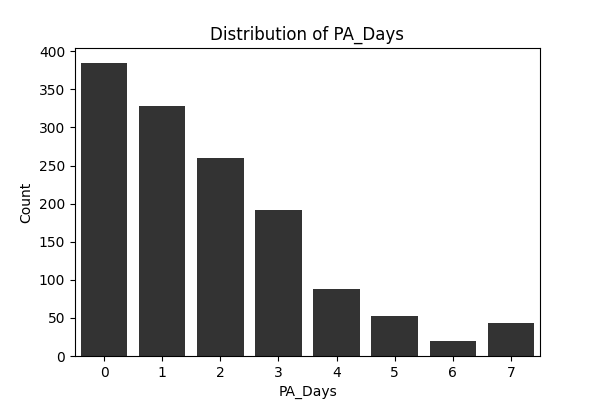
\includegraphics[width=\textwidth]{figures/pa_days_distribution.png}
        \caption{Bar chart showing the distribution of \lstinline|PA_Days| among survey participants.}
        \label{fig:pa_days}
    \end{minipage}
    \hfill
    % Second figure
    \begin{minipage}{0.48\textwidth}
        \centering
        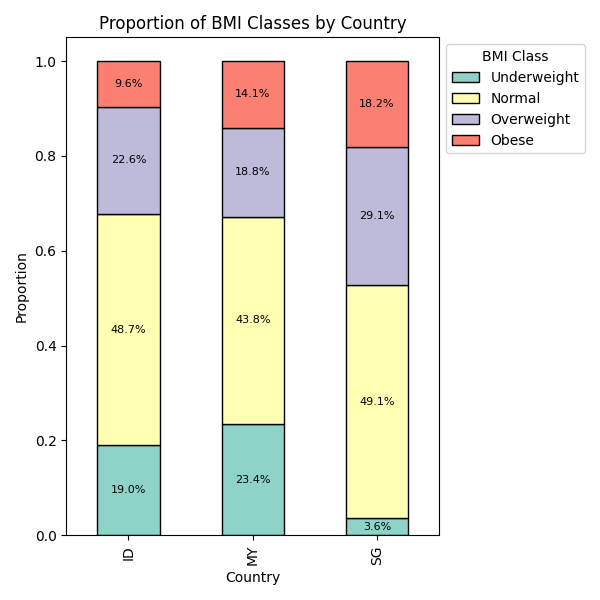
\includegraphics[width=\textwidth]{figures/bmi_class_by_country.png}
        \caption{Stacked percentage bar chart comparing the proportions of BMI class between countries.}
        \label{fig:bmi}
    \end{minipage}
\end{figure}

\lstinline|BMI| is transformed into the categorical variable \lstinline|BMI_Class| using the Asian BMI cut-off points.

From Figure~\ref{fig:bmi}, we observe that Singapore stands out with a markedly lower proportion of underweight students (only 3.6\% versus $\sim$20\% for the other two countries), and a notably higher proportion of overweight and obese students (combined 47.3\%). Malaysia has the highest proportion of underweight students (23.4\%). Indonesia's distribution is relatively balanced between categories. These differences may reflect dietary patterns, lifestyle habits, or compositional differences in the samples from each country, although the relatively small sample sizes from Singapore and Malaysia mean that these country-level comparisons should be taken with caution.

\subsection*{5. Physical Activity vs Body Weight Analysis}
\addcontentsline{toc}{subsection}{5. Physical Activity vs Body Weight Analysis}

\lstinline|MET_Daily_Hours| is a composite measure of physical activity that accounts for both the intensity and volume of activity by weighting each activity type by its metabolic equivalent: moderate intensity (4.0 METs) and vigorous intensity (8.0 METs), then multiplying by duration and frequency. This makes it a more precise and meaningful measure compared to simply counting physical activity days. This engineered feature is based on the MET minutes/week measure from the IPAQ report \cite{ipaq2004}.

\begin{figure}[h!]
    \centering
    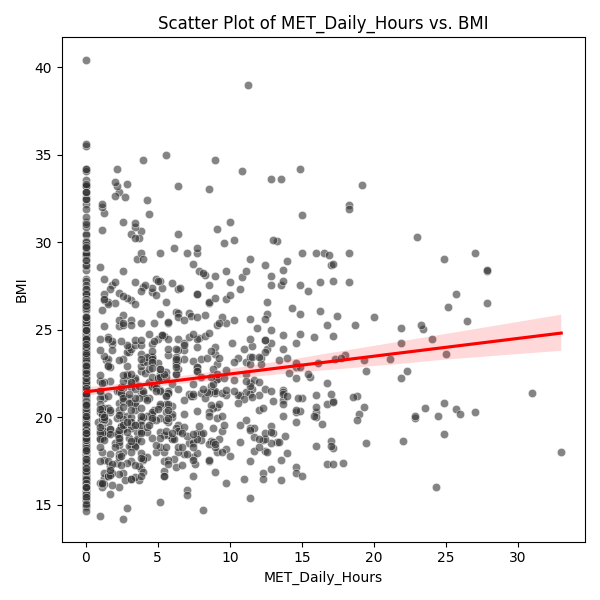
\includegraphics[width=0.45\textwidth]{figures/met_daily_hours_bmi_scatter.png}
    \caption{Scatter plot of \lstinline|MET_PA_hours| against \lstinline|BMI|, with a fitted regression line.}
    \label{fig:scatter_all}
\end{figure}

The scatter plot of \lstinline|MET_Daily_hours| versus \lstinline|BMI| in Figure~\ref{fig:scatter_all} shows a weak positive correlation ($r \approx 0.15$). Contrary to the expectation that more physical activity would correlate with lower BMI, the relationship here is positive, though the association is very weak and not practically meaningful. This may be due to the cross-sectional nature of the survey (it captures a single point in time rather than long-term habits) and the fact that BMI is influenced by many other factors not captured here (e.g., diet, genetics).

\begin{figure}[h!]
    \centering
    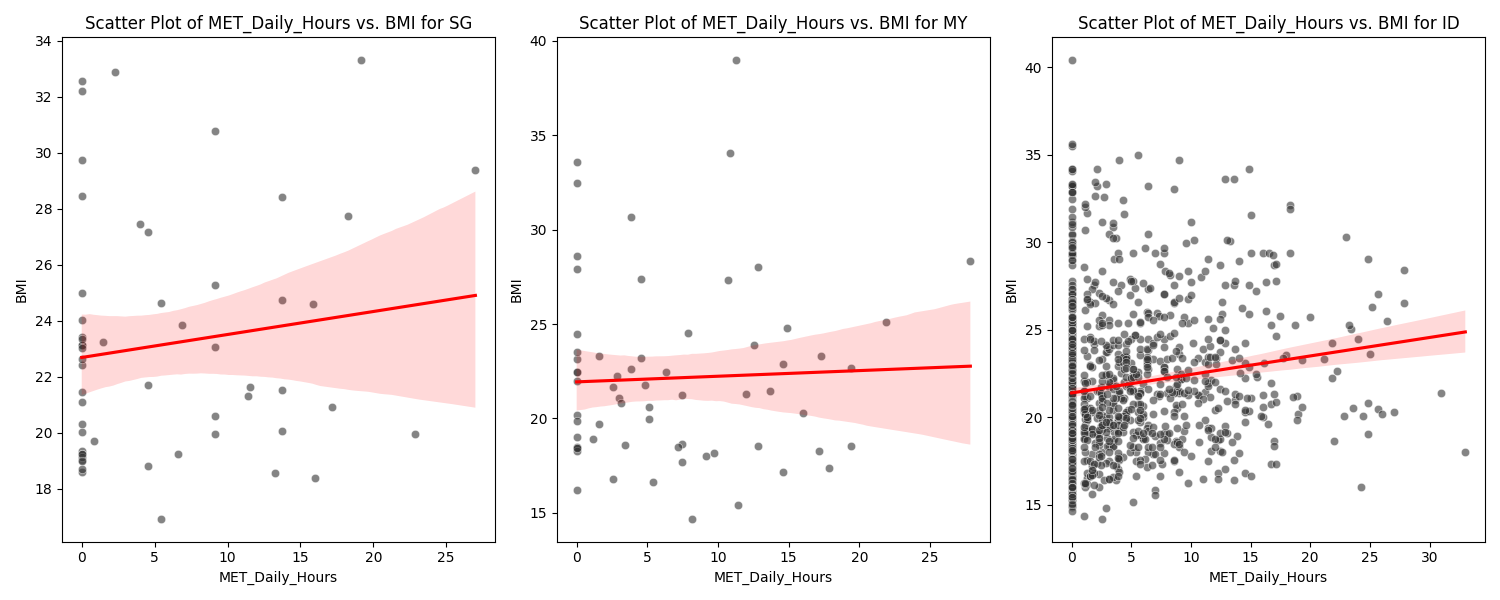
\includegraphics[width=0.95\textwidth]{figures/met_daily_hours_bmi_scatter_all.png}
    \caption{Scatter plots of \lstinline|MET_Daily_Hours| against \lstinline|BMI|, stratified by country (Singapore, Malaysia, Indonesia), each with a fitted regression line.}
    \label{fig:scatter_country}
\end{figure}

Figure~\ref{fig:scatter_country} shows that for both Singapore and Indonesia, \lstinline|MET_Daily_Hours| and \lstinline|BMI| have weak positive correlations, consistent with the overall dataset trend. However, in Malaysia, there is little to no correlation ($r = 0.04$), suggesting that unlike Singapore ($r = 0.14$) and Indonesia ($r = 0.15$), physical activity does not show any observable relationship with BMI in this sample. The overall weak relationships suggest that physical activity as measured here is not a strong predictor of BMI across this population.

\subsection*{6. Testing the Dean's Suspicions: Physical Activity}
\addcontentsline{toc}{subsection}{6. Testing the Dean's Suspicions: Physical Activity}

We use the MET (Metabolic Equivalent of Task) physical activity category as the variable to represent levels of physical activity. The criterion for categorization is based on MET minutes/week and several other PA variables. The resulting MET category classifies participants into three groups: ``inactive'', ``minimally active'', and ``HEPA active'', which are recoded as a binary variable: High PA (``HEPA active'') and Low PA (``inactive'' and ``minimally active'').

Relaxedness is recoded as: Relaxed (Relaxedness score of 4 or 5, i.e., feeling relaxed ``Often'' or ``All of the time'') and Not Relaxed (score of 1--3).

\begin{table}[h!]
\centering
\begin{tabular}{@{}llrrr@{}}
\toprule
\textbf{Group} & \textbf{PA Level} & \textbf{Not Relaxed} & \textbf{Relaxed} & \textbf{\% Relaxed} \\
\midrule
Overall & High PA & 123 & 127 & 50.8\% \\
        & Low PA  & 127 & 592 & 52.9\% \\
\midrule
Male    & High PA & 64  & 44  & 40.7\% \\
        & Low PA  & 377 & 405 & 51.8\% \\
\midrule
Female  & High PA & 59  & 83  & 58.5\% \\
        & Low PA  & 150 & 187 & 55.5\% \\
\bottomrule
\end{tabular}
\caption{Relaxedness by PA level, overall and stratified by gender.}
\label{tab:relaxedness}
\end{table}

Overall, the association between PA level and relaxedness is very weak: High PA students are marginally less likely to feel Relaxed (50.8\%) than Low PA students (52.9\%), a difference of just 2.1 percentage points that does not support the Dean's claim.

However, the gender-stratified results in Table~\ref{tab:relaxedness} reveal a striking reversal. Among males, High PA is negatively associated with relaxedness (40.7\% vs 51.8\%, a difference of 11.1 percentage points), while among females the direction flips, with High PA females marginally more likely to feel Relaxed (58.5\% vs 55.5\%). This reversal is consistent with Simpson's Paradox, and confirms that gender is a confounder: it is associated with both PA level and relaxedness, and controlling for it materially changes the observed association. The Dean's claim therefore only partially holds: the positive association between physical activity and relaxedness exists weakly among females but reverses among males.

\subsection*{7. Dean's Suspicion about Fruit Consumption among Singaporean Students}
\addcontentsline{toc}{subsection}{7. Dean's Suspicion about Fruit Consumption among Singaporean Students}

The Dean's hypothesis is that more than half of all Singaporean university students consume fewer than 2 fruits per day, which is below the Health Promotion Board (HPB's) recommendation. The null and alternative hypotheses are:
\begin{align*}
H_0&: p = 0.5, \\
H_1&: p > 0.5
\end{align*}

Among the 55 Singaporean students in the cleaned dataset, 27 (49.1\%) consumed fewer than 2 servings of fruit per day. To test the probability of observing this sample proportion or a more extreme statistic by chance, a one-tailed binomial test was conducted, yielding a $p$-value of 0.606. Therefore, we fail to reject $H_0$ at the 5\% significance level. There is insufficient evidence in this dataset to confirm the Dean's suspicion.

The observed proportion is slightly below 50\%, pointing against the Dean's claim rather than supporting it. However, there are several limitations that must be acknowledged: the sample of Singaporean university students was not specifically designed to be representative of the population of all Singaporean university students. In addition, the sample size is very small and may be insufficient to detect a small but meaningful difference from the hypothesised proportion of 0.50, potentially resulting in low statistical power. Furthermore, fruit consumption was self-reported from the survey, which may introduce recall bias or social desirability bias (overreporting of healthy eating habits); respondents may also have varying interpretations of what constitutes one serving of fruit. Thus, while the test does not support the Dean's suspicion at this significance level, the findings should be interpreted with caution. Future study may benefit from replication using a larger, more representative sample.

% ============================================================
\section*{Section 3: Thinking with Data and Reflecting on Data}
\addcontentsline{toc}{section}{Section 3: Thinking with Data and Reflecting on Data}

\subsection*{8. Additional Analysis}
\addcontentsline{toc}{subsection}{8. Additional Analysis}

Sleep is categorized into three groups: short sleep ($\leq 6$h, $n = 397$), optimal sleep (7--8h, $n = 471$), and long sleep ($\geq 9$h, $n = 501$).

\begin{figure}[h!]
        \centering
        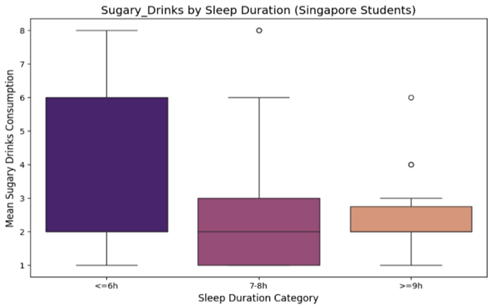
\includegraphics[width=0.75\linewidth]{figures/boxplot_sugar_consumption_sleep.png}
        \caption{Box plot of sugary drink consumption across sleep duration categories.}
        \label{fig:sugar_drinks}
    \end{figure}

Students in the $\leq 6$ hours sleep category recorded the highest median sugary drink consumption ($\approx 4$ drinks) with the widest variability (IQR: 2--6), while both the 7--8 hours and $\geq 9$ hours groups showed considerably lower medians of approximately 2 drinks and tighter distributions. This descending trend suggests that shorter sleep duration is associated with greater sugary drink consumption among Singapore students. A Chi-Square test of independence confirmed this association to be statistically significant ($\chi^2 = 27.71$, $p = 0.0156$), as the $p$-value falls below the $\alpha = 0.05$ threshold, thereby rejecting the null hypothesis that sleep duration and sugary drink consumption are independent variables.

\lstinline|BMI_Class| and sleep quality also displayed a statistically significant association, with higher BMI categories linked to poorer sleep. This suggests that weight management could be an important lever for improving sleep among university students, and points to a potential policy intervention targeting physical activity and dietary habits together with the aim of reducing excess weight and, in turn, promoting better sleep outcomes.

Regarding fruit consumption, students consuming 2 or more servings reported slightly higher proportions of optimal sleep (41.4\%) compared to those consuming fewer than 2 servings (37.7\%). However, this difference is not statistically significant ($\chi^2 = 1.76$, $p = 0.184$), so we fail to reject the null hypothesis of independence. There is insufficient evidence to conclude that fruit consumption is associated with sleep quality.

\subsection*{9. Proposed Variable to Collect}
\addcontentsline{toc}{subsection}{9. Proposed Variable to Collect}

We would propose the Pittsburgh Sleep Quality Index (PSQI) \cite{buysse1989} to measure the sleep quality of university students. The PSQI is a validated self-report tool measuring overall sleep quality across 7 components, making it directly relevant to university student health. It asks respondents to reflect on their sleep habits over the past month. While the existing dataset captures sleep duration, this alone is insufficient. Two students sleeping the same number of hours may have vastly different sleep quality due to differences in sleep efficiency, disturbances, or daytime dysfunction. The PSQI addresses this gap by measuring sleep as a multidimensional construct, accounting for individual variation in sleep needs and capturing aspects of sleep health that duration simply cannot reflect.

\textit{Measurement.} Students complete 19 items covering sleep duration, efficiency, disturbances, and daytime dysfunction, producing a global score from 0--21 (above 5 = poor sleep quality). It takes 5--10 minutes and can be embedded directly into a survey, requiring no external monitoring devices.

\textit{Limitations.} As a self-report measure, PSQI responses are susceptible to recall and social desirability bias, where students may underreport sleep problems or misremember sleep patterns from the past month. Additionally, the PSQI captures average patterns over 30 days, so it may not reflect acute disruptions like exam periods, which are especially relevant for university students.

\subsection*{10. Evaluation of Data Analysis (Part B)}
\addcontentsline{toc}{subsection}{10. Evaluation of Data Analysis (Part B)}

\subsubsection*{Aspect 1: MET Activity.}
The use of MET-minutes per week as the primary measure of physical activity significantly adds value to the understanding of the relationship between physical activity and sleep duration. Rather than treating all active days as equal, MET-minutes captures both the intensity and volume of activity by applying weighted MET values. This allows for more accurate PA Level classification, which is more meaningful in the context of sleep research, as it enables the analysis to detect whether it is the degree of physical exertion, and not the frequency of activity, that is associated with differences in sleep duration.

A limitation of this analysis is that the physical activity data is derived from the IPAQ short-form questionnaire, which relies entirely on self-reporting. Respondents are required to recall the frequency and duration of their physical activities over the past week, which is susceptible to recall bias and social desirability bias, where participants may overestimate their activity levels.

\subsubsection*{Aspect 2: Generalisability of Findings.}
In Part B, apart from Questions 7 and 8, the full sample was used for the analysis. However, the dataset is heavily skewed towards Indonesian students, who account for approximately 89\% of the cleaned sample, while Singapore contributes only around 4\%. This severe imbalance means that the overall findings are largely driven by the Indonesian subgroup and may not accurately reflect the health behaviours of NUS students specifically. Furthermore, the data were collected during the COVID-19 pandemic (March--June 2021), when movement restrictions and campus closures were in effect across all participating countries, likely suppressing typical physical activity levels and altering dietary and sleep habits. As such, there is a large discrepancy between the population of interest (NUS university students) and the sampling frame.